\documentclass[12pt,border=4pt,multi]{article} % \documentclass[tikz,border=4pt,multi]{article}
\usepackage{lingmacros}
\usepackage{tree-dvips}
\usepackage{amssymb} % for mathbb{}
\usepackage[dvipsnames]{xcolor}
\usepackage{forest}
\usepackage{amsmath} % for matrices
\usepackage{xeCJK}
\usepackage{tikz}
\usepackage[arrowdel]{physics}
\usepackage{graphicx}
\usepackage{wrapfig}
\usepackage{listings}
\usepackage{pgfplots, pgfplotstable}
\usepackage{diagbox} % diagonal line in cell
\usepackage[usestackEOL]{stackengine}
\usepackage{multirow}
\graphicspath{{./img}} % specify the graphics path to be relative to the main .tex file, denoting the main .tex file directory as ./
\definecolor{orchid}{rgb}{0.7, 0.4, 1.1}

\begin{document}
\section*{Xi Liu, xl3504, Homework 9}
Problem 1\\
let $G_1$ be a set containing some vertices of $G$\\
    $G_2$ be a set containing some vertices of $G$\\
let there be an edge from a vertex in set $G_2$ to vertex $v$ and an edge from vertex $v$ to a vertex in set $G_1$ as shown below, then if all of the vertices in set $G_1$ are visited before visiting $v$, then there is no outgoing edge of $v$ remaining to visit, so if $v$ is chosen to be visited next, it will be the only vertex in the DFS tree\\
\begin{figure}[h!]
	\centering
	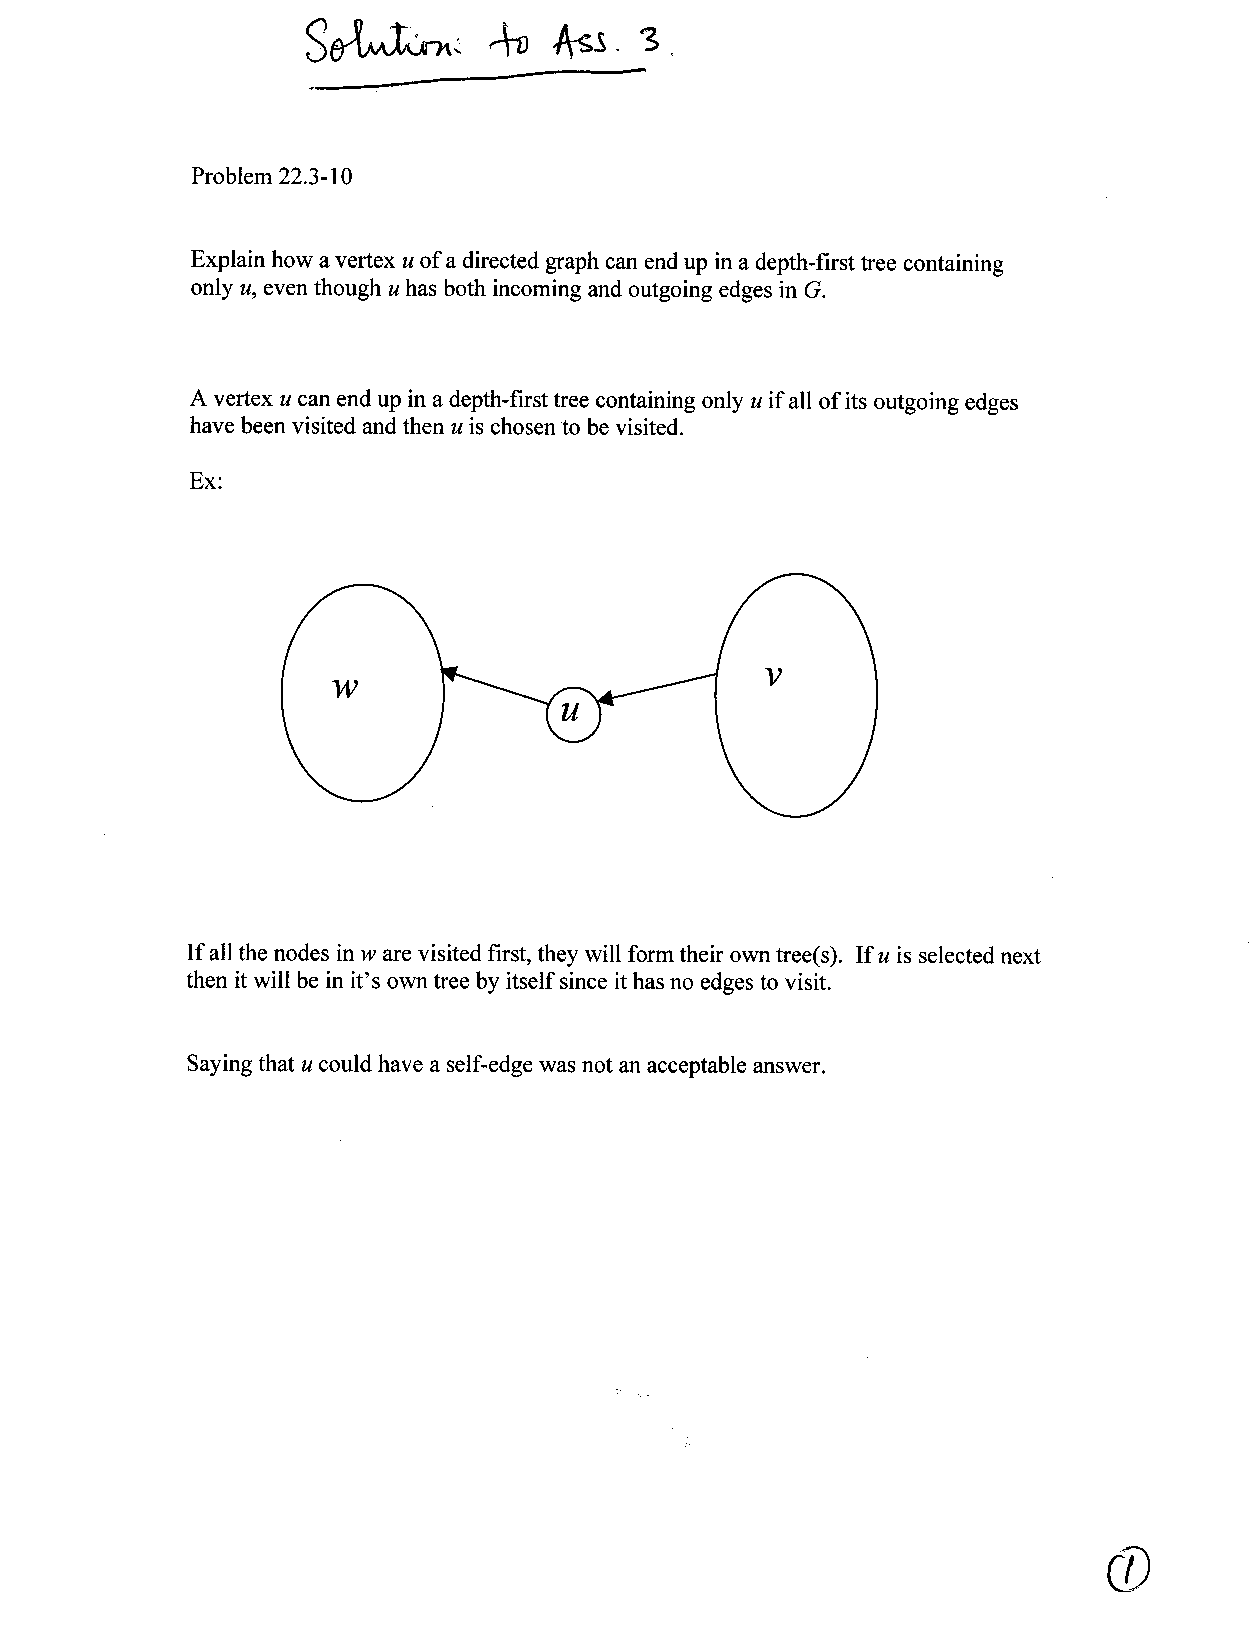
\includegraphics[width=1.1\textwidth, height=0.55\textwidth]{1} %img size
\end{figure}\\
\newpage
\noindent
Problem 2\\
has\_cycle() is an algorithm that determines whether G has a
cycle, has\_cycle()'s time complexity is $O(|V| + |E|)$ since has\_cycle() calls the recursive function has\_back\_edge() only when $!visited[i]$ which means the vertex has not been visited before. it finds a back edge when there is a vertex $i$ that is adjacent to $v$ and is visited but $i$ is the descendant of the current vertex $v$ (equivalently $i$ is not the parent of $v$), descendant.discovery\_time $<$ ancestor.discovery\_time \\
\begin{lstlisting}[language = c++]
#include <stdio.h>
#include <stdlib.h>
#include <string.h>
#include <list>
using namespace std;

struct graph 
{
    int n_v;
    bool * visited;
    list<int> * adj;
    graph(int n_v);
    void clear_visit();
    void add_edge(int v1, int v2);
    bool has_back_edge(int v, int parent);
    bool has_cycle();
};

graph::graph(int n_v)
{
    this->n_v = n_v;
    adj = new list<int>[n_v];
    visited = (bool *)malloc(n_v * sizeof(bool));
}

void graph::clear_visit()
{
    memset(visited, false, n_v * sizeof(bool));
}
 
void graph::add_edge(int v1, int v2)
{
    adj[v1].push_back(v2);
    adj[v2].push_back(v1);
}

bool graph::has_back_edge(int v, int parent)
{
    visited[v] = true;
    for(list<int>::iterator i = adj[v].begin(); i != adj[v].end(); ++i)
    {
        if(!visited[*i])
        {
            if(has_back_edge(*i, v))
                return true;
        }
        else if(visited[*i])
        {
            if(*i != parent) /* for an edge between 
            {ancestor, descendant}, 
            descendant.discovery_time < ancestor.discovery_time */
                return true;
        }
    }
    return false;
}

bool graph::has_cycle()
{
    clear_visit();
    for(int i = 0; i < n_v; ++i)
    {
        if(!visited[i])
            if(has_back_edge(i, -1))
                return true;
    }
    return false;
}
\end{lstlisting}
\newpage
\noindent
Problem 3\\
(a)\\
graph with vertices $\{v_1, v_2, u, v\}$ have edges $(v_1, v_2), (v_2, u), (u, v_1), (v_1, v)$ as shown below, there is a path from $u$ to $v$ through $u \rightarrow v_1 \rightarrow v$\\
$u.d = 3 < v.d = 6$ in depth-first search of $G$\\
\begin{figure}[h!]
	\centering
	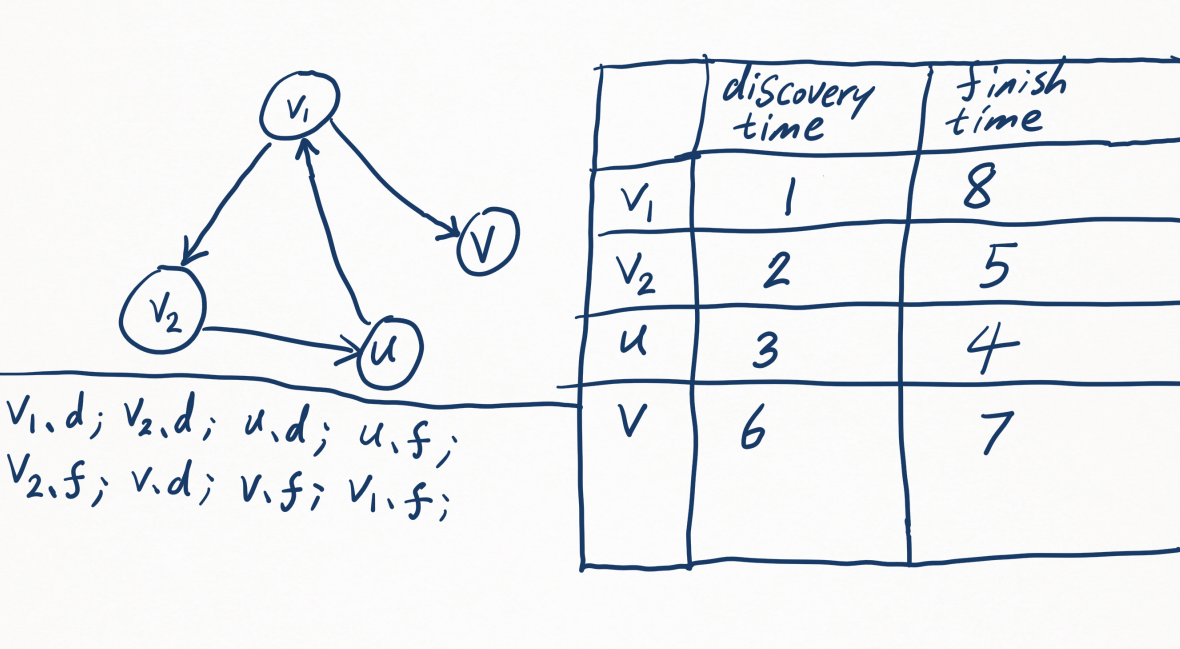
\includegraphics[width=1.1\textwidth, height=0.65\textwidth]{3a} %img size
\end{figure}
\\
in the depth-first forest generated below for $G$, $v$ is not a descendant of $u$
\begin{figure}[h!]
	\centering
	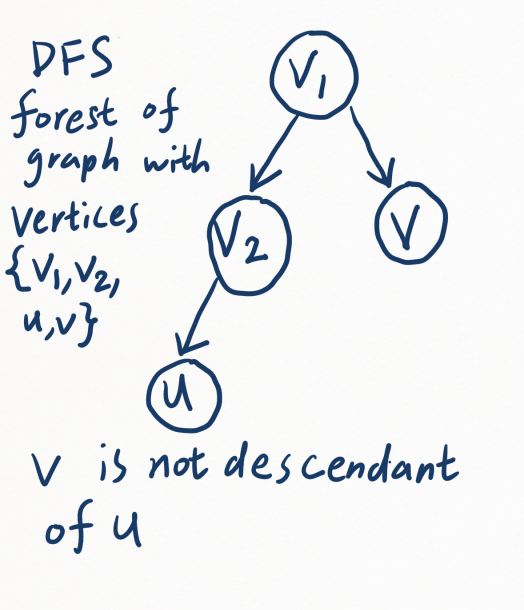
\includegraphics[width=0.7\textwidth, height=0.75\textwidth]{3a2} %img size
\end{figure}
\newpage
\noindent
\\
\\
\\
\\
(b)\\
graph with vertices $\{a, b, u, v\}$ have edges $(a, u), (u, a), (a, v), (a, b)$ as shown below, there is a path from $u$ to $v$ through $u \rightarrow a \rightarrow v$\\
$v.d \not\leq u.f$ since $v.d = 4 > u.f = 3$ in depth-first search of $G$\\
\begin{figure}[h!]
	\centering
	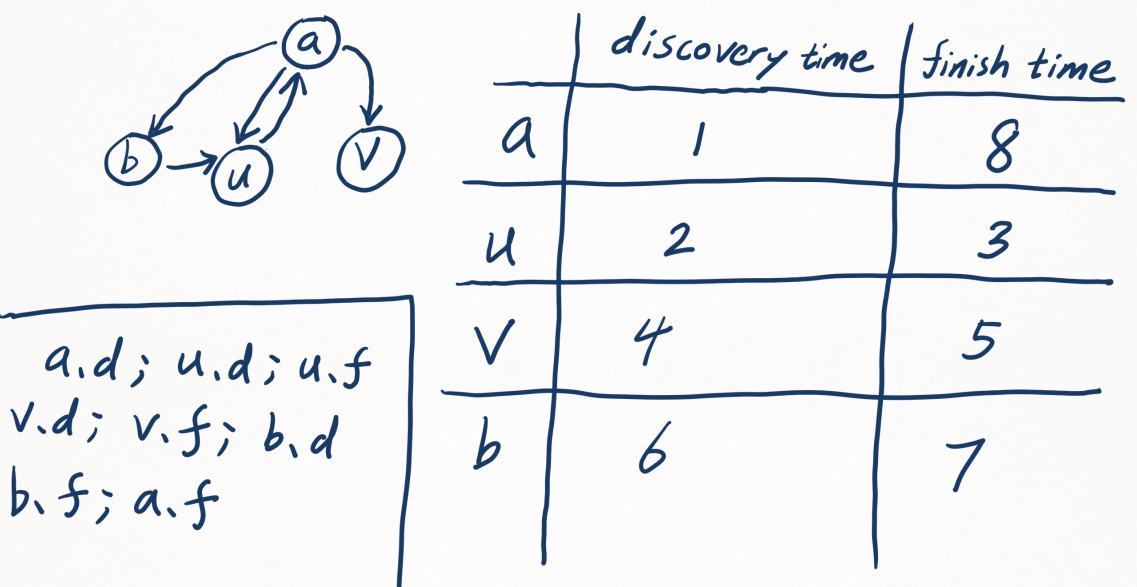
\includegraphics[width=1.1\textwidth, height=0.65\textwidth]{3b} %img size
\end{figure}
\begin{figure}[h!]
	\centering
	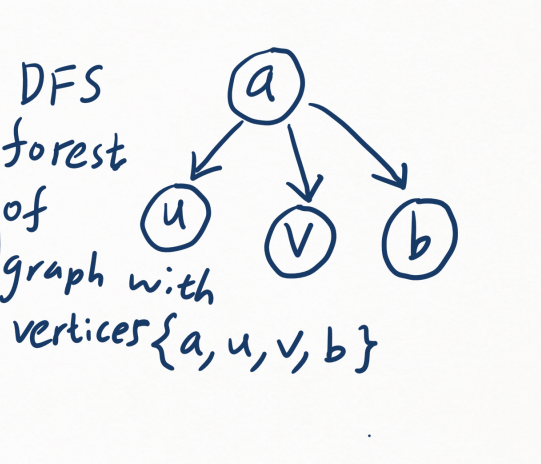
\includegraphics[width=0.7\textwidth, height=0.75\textwidth]{3b2} %img size
\end{figure}
\\
\\
\\
\\
\newpage
\noindent
\\
\newpage
\noindent
\\
\newpage
\noindent
Problem 4\\
algorithm:\\
stage 1:\\
let $G_{red}$ be a graph containing only red edges\\ 
$G_{blue}$ be a graph containing only blue edges\\
$G_{red} = (V, E_{red})$, in which $V$ is the set containing all vertices in $G$; $E_{red}$ is the set containing red edges of $G$\\
$G_{blue} = (V_{cp}, E_{blue\_cp})$, in which $V_{cp}$ contains the copies of all vertices in $V$; $E_{blue\_cp}$ is the set containing blue edges that connects each vertex in $V_{cp}$ instead of each vertex in $V$\\
denote each vertex $v \in V$ and each vertex in $v_{cp} \in V_{cp}$ with an index such that
\begin{align*}
V &= \bigcup_{i = 0}^{|V| - 1} \{v_i\}\\
V_{cp} &= \bigcup_{i = 0}^{|V| - 1} \{v_{cp\_i}\}\\
&v_{cp\_i}\text{ is a copy of }v_i\\
\end{align*}
\\
\\
stage 2:\\
call a vertex a transitional vertex if there exist at least an incoming  edge going into the vertex and at least an outgoing edge coming out of the vertex. to find transitional vertices, allocate a 2 dimensional array $trans$ that has 2 rows and $|V|$ columns, where 
\begin{lstlisting}[language = c++]
bool trans[2][|V|];
memset(trans, false, sizeof(trans));
\end{lstlisting}
$\forall idx \in [0, |V| - 1] \cap \mathbb{N}\\
trans[0][idx] = 
\begin{cases}
\text{true} & \text{if vertex } v_{idx} \text{ has an incoming red edge}\\
\text{false} & \text{otherwise}\\
\end{cases}\\
trans[1][idx] = 
\begin{cases}
\text{true} & \text{if vertex } v_{idx} \text{ has an outgoing blue edge}\\
\text{false} & \text{otherwise}\\
\end{cases}$\\
\\
\\
stage 3:
\begin{lstlisting}[language = c++, mathescape = true]
for each directed edge $(v_i, v_j) \in G.E$
{
    if($(v_i, v_j)$ is a red edge)
        trans[0][j] = true;
    if($(v_i, v_j)$ is a blue edge)
        trans[1][i] = true;
}
\end{lstlisting}
\leavevmode
\\
\\
stage 4:
\begin{lstlisting}[language = c++, mathescape = true]
vector<edge> $E_{pink}$;
for(int j = 0; j < |V|; ++j)
{
    if(trans[0][j] && trans[1][j])
    {
        edge new_pink_edge = new pink edge ($v_j, v_{cp\_j}$);
        $E_{pink}$.push_back(new_pink_edge);
    }
}
$E_{pink}$.push_back(new pink edge ($s$, copy of $s$));
$E_{pink}$.push_back(new pink edge ($t$, copy of $t$));
\end{lstlisting}
\leavevmode
\\
\\
stage 5:\\
let $G_{big} = \{V \cup V_{cp},\;\; E_{red} \cup E_{blue} \cup E_{pink}\}$\\
use function $P$ with to find the shortest path from vertex $s$ to $t_{cp}$, then output a sequence of edges or a sequence of vertices, assume the output is a sequence of vertices\\
\\
\\
stage 6:\\
traverse through the sequence of vertices, keep track of the vertex immediately before the current vertex, then if the previous vertex and the current vertex forms a pair of $v_i$ and $v_{cp\_i}$, then this is a pink edge that we created, so remove the pink edge; and during the traversal, replace every vertex $v_{cp\_i} \in V_{cp}$ with its corresponding vertex $v_i \in V$. then output the modified sequence that is the shortest path from vertex $s$ to $t$\\
\\
\\
time complexity:\\
$T(\text{stage 1}) = |E| + |V|$; traverse through edges and separate them into the red graph and the blue graph takes $|E|$. then $|V|$ is required to create the copies $v_{cp\_i} \in V_{cp}$\\
\\
$T(\text{stage 2}) = 1$; allocate a 2 dimensional array $trans$ and initialize it requires constant time\\
\\
$T(\text{stage 3}) = |E|$; traverse all edges and marking them as either red or blue in the 2 dimensional array $trans$, each mark requires constant time\\
\\
$T(\text{stage 4}) = |V| + 2$; for loop has number of iterations equal to $|V|$ and each iteration requires constant if tests; in addition, 2 pink edges $(s, \text{ copy of } s), (t, \text{ copy of } t)$ are added to the $E_{pink}$ set\\ 
\\
$T(\text{stage 5}) = O(|E|) + T(P)$; create the new graph $G_{big}$ potentially requires allocating a new adjacency list and then copying all edges in $E_{red} \cup E_{blue} \cup E_{pink}$ to $G_{big}$'s adjacency list which may take $O(|E|)$, then 1 call to $P$ takes $T(P)$\\
\\
$T(\text{stage 6}) = O(|E|)$; traversing the the optimal path output of $P$ for which its number of edges is at most $O(|E|)$\\
\\
\begin{align*}
\text{total time complexity} &= \sum_{i = 1}^6 (\text{stage } i)\\
&= |E| + |V| + 1 + |E| + |V| + 2 + O(|E|) + T(P) + O(|E|)\\
&= O(|E| + |V|) + T(P)\\
\end{align*}
\end{document}